\documentclass[aspectratio=169]{beamer}

\usetheme{Frankfurt}
\setbeamertemplate{navigation symbols}{}
\setbeamertemplate{footline}[frame number]

\usepackage{amsmath}
\usepackage{booktabs}
\usepackage{graphicx}
\graphicspath{{Exps/}}
\usepackage{tikz}
\usetikzlibrary{arrows.meta,positioning,calc}

\definecolor{kepblue}{RGB}{42,88,140}
\definecolor{kepteal}{RGB}{33,132,120}
\definecolor{keporange}{RGB}{210,122,39}
\definecolor{kepred}{RGB}{178,61,68}
\definecolor{kepgray}{RGB}{92,99,112}

\setbeamercolor{structure}{fg=kepblue}
\setbeamercolor{block title}{bg=kepblue!12,fg=kepblue!90!black}
\setbeamercolor{block body}{bg=kepblue!4,fg=black}
\setbeamercolor{alerted text}{fg=kepred}

\title{Decision-Focused Learning for Kidney Exchange Programs}
\subtitle{Internship Research Project}
\author{Weikang Fu}
\institute{MILA\\Universit\'{e} de Montr\'{e}al}
\date{\today}

\newcommand{\G}{\mathcal{G}}
\newcommand{\V}{\mathcal{V}}
\newcommand{\A}{\mathcal{A}}
\newcommand{\E}{\mathcal{E}}
\newcommand{\R}{\mathbb{R}}

\tikzset{
  block/.style={
    draw=kepblue!70,
    fill=kepblue!6,
    rounded corners=2pt,
    align=center,
    minimum height=8mm,
    text width=22mm,
    font=\small
  },
  smallblock/.style={
    draw=kepgray!70,
    fill=kepgray!7,
    rounded corners=2pt,
    align=center,
    minimum height=7mm,
    text width=18mm,
    font=\scriptsize
  },
  pair/.style={
    circle,
    draw=kepblue!80,
    fill=kepblue!8,
    minimum size=9mm,
    inner sep=1pt,
    font=\scriptsize
  },
  ndd/.style={
    circle,
    draw=kepteal!90!black,
    fill=kepteal!10,
    minimum size=9mm,
    inner sep=1pt,
    font=\scriptsize
  },
  arr/.style={-Latex,thick,kepblue!85},
  highlightarr/.style={-Latex,very thick,keporange}
}

\begin{document}

\begin{frame}
  \titlepage
\end{frame}

\section{Motivation}

\begin{frame}{Why Kidney Exchange Matters}
  \begin{columns}[T,onlytextwidth]
    \begin{column}{0.52\textwidth}
      \begin{itemize}
        \item Many patients need kidney transplants, but compatible living donors are scarce.
        \item A willing donor may be medically incompatible with the intended recipient.
        \item Kidney exchange pools incompatible pairs and selects swaps.
        \item Non-directed donors can start chains that help multiple patients.
      \end{itemize}
    \end{column}
    \begin{column}{0.46\textwidth}
      \centering
      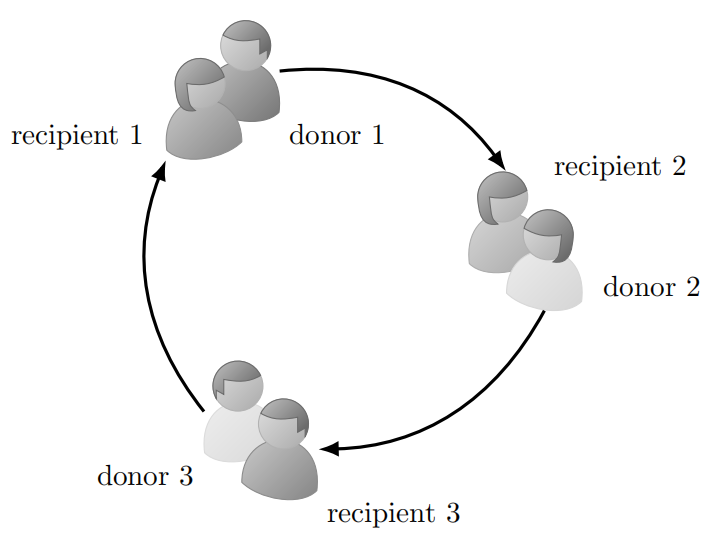
\includegraphics[width=\linewidth,height=0.31\textheight,keepaspectratio]{figures/intern01/kep_cycle.png}\\[-0.2em]
      {\footnotesize\textbf{Cycle}}\\[0.5em]
      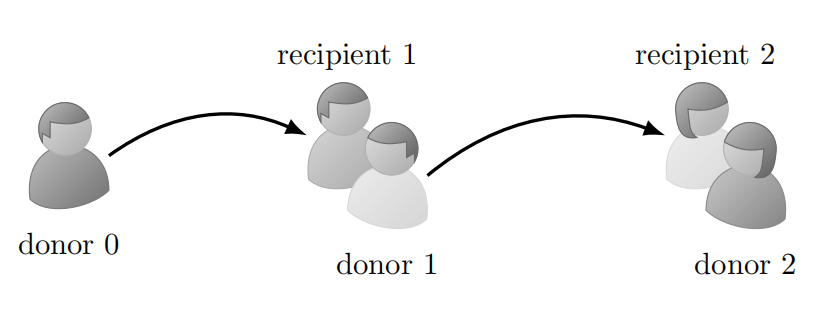
\includegraphics[width=\linewidth,height=0.24\textheight,keepaspectratio]{figures/intern01/kep_chain.png}\\[-0.2em]
      {\footnotesize\textbf{Chain}}
    \end{column}
  \end{columns}
\end{frame}

\begin{frame}{Kidney Exchange as a Graph Optimization Problem}
  \footnotesize
  \begin{columns}[T,onlytextwidth]
    \begin{column}{0.47\textwidth}
      \begin{itemize}
        \item \textbf{Sets:}
        \(\mathcal{R}\): recipient--donor pairs,
        \(\mathcal{N}\): non-directed donors.

        \item \textbf{Graph:}
        \(G=(\V,\A)\), with vertices
        \(\V=\mathcal{R}\cup\mathcal{N}\).

        \item \textbf{Limits:}
        \(K\): maximum cycle length,
        \(L\): maximum chain length.

        \item \textbf{Cycle:}
        \(\langle v_1,\dots,v_k,v_1\rangle\),
        \(k\le K\), using distinct vertices in \(\mathcal{R}\).

        \item \textbf{Chain:}
        starts from \(n\in\mathcal{N}\), then visits compatible pairs,
        with length at most \(L\).

        \item \textbf{Goal:}
        select vertex-disjoint cycles and chains maximizing total edge weight \(w_{uv}\).
      \end{itemize}
    \end{column}
    \begin{column}{0.51\textwidth}
      \centering
      \resizebox{\linewidth}{!}{%
      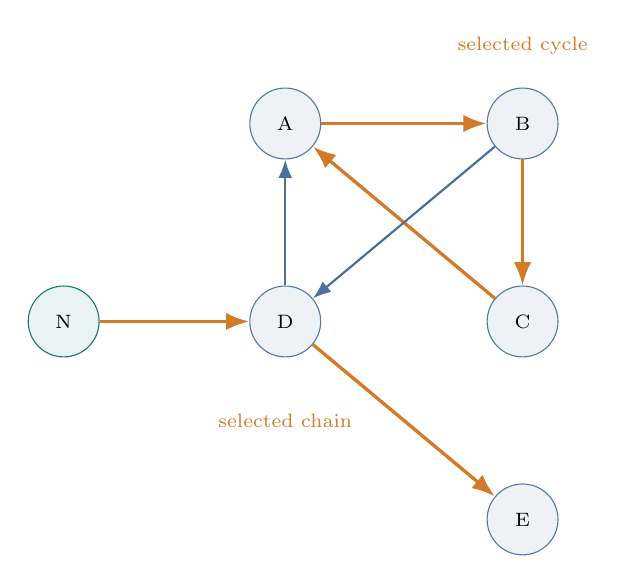
\begin{tikzpicture}[node distance=16mm]
        \node[pair] (a) {A};
        \node[pair,right=21mm of a] (b) {B};
        \node[pair,below=16mm of b] (c) {C};
        \node[pair,below=16mm of a] (d) {D};
        \node[ndd,left=19mm of d] (n) {N};
        \node[pair,below=16mm of c] (e) {E};

        \draw[highlightarr] (a) -- (b);
        \draw[highlightarr] (b) -- (c);
        \draw[highlightarr] (c) -- (a);

        \draw[arr] (d) -- (a);
        \draw[arr] (b) -- (d);
        \draw[highlightarr] (n) -- (d);
        \draw[highlightarr] (d) -- (e);

        \node[font=\scriptsize,keporange,above=3mm of b] {selected cycle};
        \node[font=\scriptsize,keporange,below=6mm of d] {selected chain};
      \end{tikzpicture}
      }
    \end{column}
  \end{columns}
\end{frame}

\begin{frame}{Example}
  \scriptsize
  \begin{columns}[T,onlytextwidth]
    \begin{column}{0.35\textwidth}
      \centering
      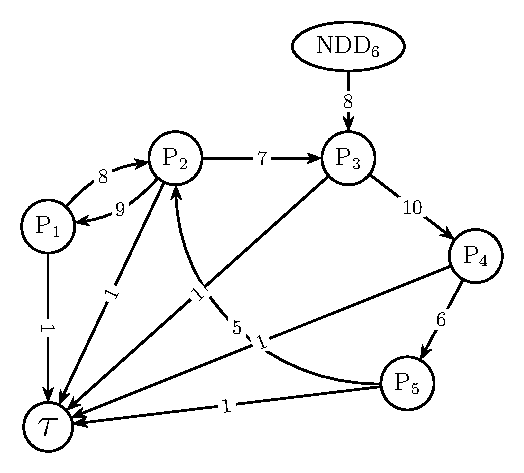
\includegraphics[width=\linewidth,height=0.72\textheight,keepaspectratio]{figures/intern01/kep_example.pdf}
    \end{column}

    \begin{column}{0.65\textwidth}
      \textbf{Instance.}
      \[
        \mathcal{R}=\{P_1,P_2,P_3,P_4,P_5\},\quad
        \mathcal{N}=\{\mathrm{NDD}_6\},\quad K=4,\quad L=4.
      \]

      \vspace{0.2em}
      \textbf{Possible Cycles (RDP-only closed loops)}
      \begin{itemize}\setlength{\itemsep}{1pt}
        \item Cycle 1 (2-way): \(P_1 \to P_2 \to P_1\); length 2.
        \item Cycle 2 (4-way): \(P_2 \to P_3 \to P_4 \to P_5 \to P_2\); length 4.
      \end{itemize}

      \vspace{0.2em}
      \textbf{Possible Chains (start at NDD, end at \(\tau\))}
      \begin{itemize}\setlength{\itemsep}{1pt}
        \item Chain 1: \(\mathrm{NDD}_6 \to P_3 \to \tau\); length 2.
        \item Chain 2: \(\mathrm{NDD}_6 \to P_3 \to P_4 \to \tau\); length 3.
        \item Chain 3: \(\mathrm{NDD}_6 \to P_3 \to P_4 \to P_5 \to \tau\); length 4.
        \item Chain 4: \(\mathrm{NDD}_6 \to P_3 \to P_4 \to P_5 \to P_2 \to \tau\); length 5.
        \item Chain 5: \(\mathrm{NDD}_6 \to P_3 \to P_4 \to P_5 \to P_2 \to P_1 \to \tau\); length 6.
      \end{itemize}
    \end{column}
  \end{columns}
\end{frame}

\begin{frame}{What Makes the Problem Difficult?}
  \large
  \textbf{Two difficulties:}

  \vspace{0.8em}
  \begin{enumerate}
    \item \textbf{Optimization difficulty}
    \begin{itemize}
      \item Cycles/chains create a combinatorial problem.
      \item Bounded cycle length \(>2\) is NP-hard.
    \end{itemize}

    \vspace{0.8em}
    \item \textbf{Prediction difficulty}
    \begin{itemize}
      \item The benefit of a transplant edge is uncertain.
      \item A good edge-level prediction may not lead to the best final exchange plan.
    \end{itemize}
  \end{enumerate}
\end{frame}

\section{Learning Problem}

\begin{frame}{From Transplant Benefit to Edge Weights}
  \small
  Each possible transplant edge needs a benefit score.

  \vspace{0.8em}
  \begin{columns}[T,onlytextwidth]
    \begin{column}{0.36\textwidth}
      \textbf{Clinical benefit components}
      \begin{itemize}\setlength{\itemsep}{0.35em}
        \item transplant success probability
        \item Quality-Adjusted Life Year (QALY)
        \item fairness or priority terms
        \item patient-donor compatibility quality
      \end{itemize}
    \end{column}

    \begin{column}{0.24\textwidth}
      \centering
      \vspace{0.2em}
      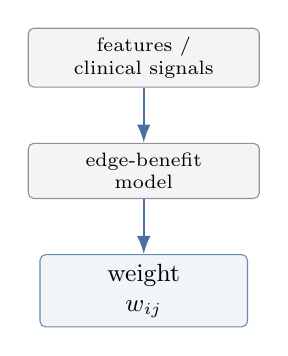
\begin{tikzpicture}[node distance=7mm]
        \node[smallblock,text width=27mm] (signals) {features /\\clinical signals};
        \node[smallblock,below=of signals,text width=27mm] (model) {edge-benefit\\model};
        \node[block,below=of model,text width=24mm] (weight) {weight\\\(w_{ij}\)};
        \draw[arr] (signals) -- (model);
        \draw[arr] (model) -- (weight);
      \end{tikzpicture}
    \end{column}

    \begin{column}{0.36\textwidth}
      \textbf{What the optimizer sees}
      \begin{itemize}\setlength{\itemsep}{0.45em}
        \item a weighted compatibility graph
        \item edge \(i\to j\) has scalar weight \(w_{ij}\)
        \item cycles/chains are selected using these weights
      \end{itemize}

      \vspace{0.4em}
      \[
        i\to j \quad \leadsto \quad w_{ij}
      \]
    \end{column}
  \end{columns}
\end{frame}

\begin{frame}{Standard Approach: Predict Then Optimize}
  \small

  \vspace{0.2em}
  \centering
  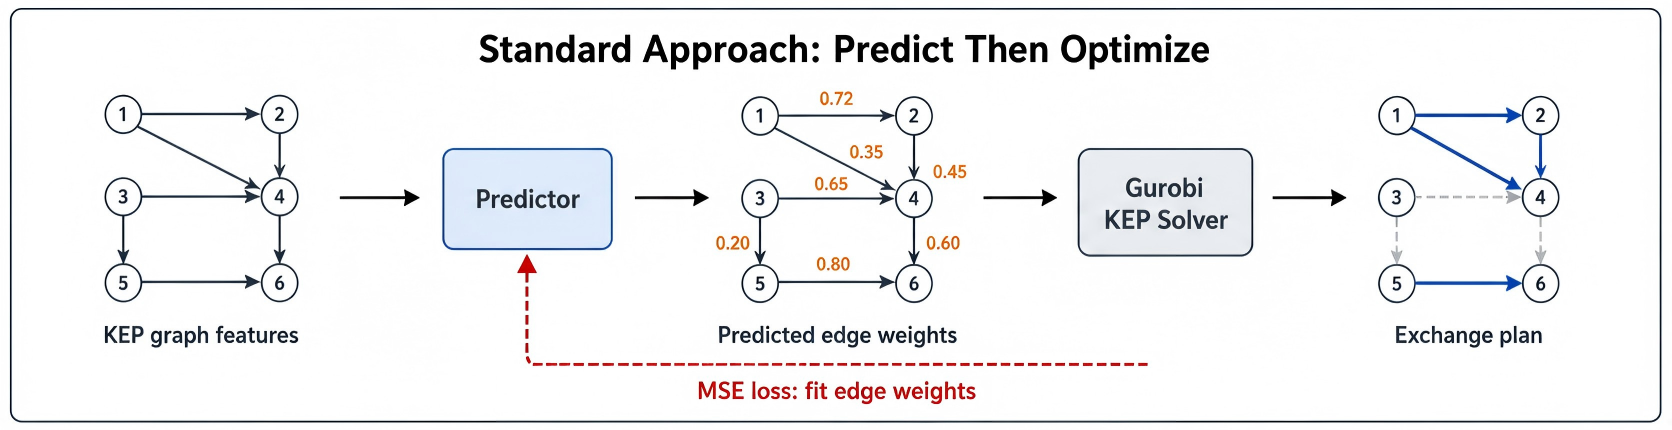
\includegraphics[width=0.98\textwidth]{figures/intern01/Standard Approach.png}

  \vspace{0.1em}
  \begin{columns}[T,onlytextwidth]
    \begin{column}{0.48\textwidth}
      \begin{block}{Step 1: train ML model}
        \centering
        features \(\longrightarrow\) predicted edge weights
      \end{block}
    \end{column}
    \begin{column}{0.48\textwidth}
      \begin{block}{Step 2: run KEP optimizer}
        \centering
        predicted weights \(\longrightarrow\) selected cycles/chains
      \end{block}
    \end{column}
  \end{columns}

  \vspace{0.35em}
  \begin{alertblock}{Problem}
    \centering
    Prediction loss \(\neq\) decision quality.
  \end{alertblock}
\end{frame}

\begin{frame}{Research Idea: Learning for the Final Exchange Plan}
  \footnotesize
  \begin{columns}[T,onlytextwidth]
    \begin{column}{0.54\textwidth}
      \textbf{Core idea}
      \begin{itemize}\setlength{\itemsep}{0.25em}
        \item We care about the final KEP decision gap.
        \item But the discrete solver is not directly differentiable.
        \item Train the reward model with a decision-focused surrogate.
      \end{itemize}

      \vspace{0.45em}
      \textbf{Questions}
      \begin{itemize}\setlength{\itemsep}{0.25em}
        \item Can surrogate training reduce the decision gap compared with MSE?
        \item Does the improvement generalize to held-out or unseen KEP graphs?
        \item When does the surrogate advantage disappear?
      \end{itemize}
    \end{column}

    \begin{column}{0.45\textwidth}
      \centering
      \textbf{Prediction accuracy \(\neq\) decision quality}

      \vspace{0.5em}
      \begin{columns}[T,totalwidth=\linewidth]
        \begin{column}{0.49\linewidth}
          \centering
          {\scriptsize Predicted weights}

          \vspace{0.2em}
          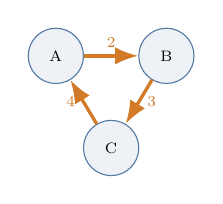
\begin{tikzpicture}[scale=0.78, every node/.style={transform shape}]
            \node[pair] (a) at (0,1.5) {A};
            \node[pair] (b) at (1.8,1.5) {B};
            \node[pair] (c) at (0.9,0) {C};
            \draw[highlightarr] (a) -- node[above,font=\scriptsize] {2} (b);
            \draw[highlightarr] (b) -- node[right,font=\scriptsize] {3} (c);
            \draw[highlightarr] (c) -- node[left,font=\scriptsize] {4} (a);
          \end{tikzpicture}
        \end{column}

        \begin{column}{0.49\linewidth}
          \centering
          {\scriptsize Same weights \(\times 5\)}

          \vspace{0.2em}
          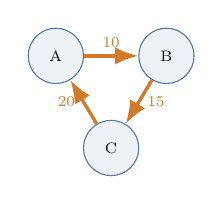
\begin{tikzpicture}[scale=0.78, every node/.style={transform shape}]
            \node[pair] (a) at (0,1.5) {A};
            \node[pair] (b) at (1.8,1.5) {B};
            \node[pair] (c) at (0.9,0) {C};
            \draw[highlightarr] (a) -- node[above,font=\scriptsize] {10} (b);
            \draw[highlightarr] (b) -- node[right,font=\scriptsize] {15} (c);
            \draw[highlightarr] (c) -- node[left,font=\scriptsize] {20} (a);
          \end{tikzpicture}
        \end{column}
      \end{columns}

      \vspace{1em}
      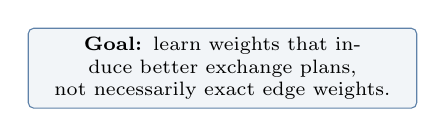
\begin{tikzpicture}
        \node[smallblock,text width=47mm,draw=kepblue!75,fill=kepblue!6] {
          \textbf{Goal:} learn weights that induce better exchange plans, \\
          not necessarily exact edge weights.
        };
      \end{tikzpicture}
    \end{column}
  \end{columns}
\end{frame}

\begin{frame}{Why End-to-End Training Is Hard}
  \footnotesize
  \centering
  \textit{The right objective is the final decision gap, but it is not an easy training signal.}

  \vspace{0.8em}
  \begin{columns}[T,onlytextwidth]
    \begin{column}{0.48\textwidth}
      \textbf{\textcolor{kepred}{Challenge 1: Non-differentiability}}
      \begin{itemize}\setlength{\itemsep}{0.35em}
        \item The KEP solver returns a discrete exchange plan.
        \item Small changes in predicted weights may not change the selected plan.
        \item The true decision gap has zero or undefined gradients.
      \end{itemize}
    \end{column}

    \begin{column}{0.48\textwidth}
      \textbf{\textcolor{keporange}{Challenge 2: Computational cost}}
      \begin{itemize}\setlength{\itemsep}{0.35em}
        \item Training now calls the KEP solver inside the learning loop.
        \item Perturbation-based surrogates require many repeated solver calls.
        \item Full end-to-end training is much more expensive than MSE.
      \end{itemize}
    \end{column}
  \end{columns}

  \vspace{1.1em}
  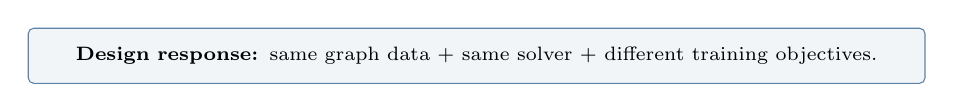
\begin{tikzpicture}
    \node[smallblock,text width=0.92\textwidth,draw=kepblue!75,fill=kepblue!6] {
      \textbf{Design response:} same graph data + same solver + different training objectives.
    };
  \end{tikzpicture}
\end{frame}

\section{Experiments}

\begin{frame}{Research Approach: Experimental Pipeline}
  \scriptsize
  \centering
  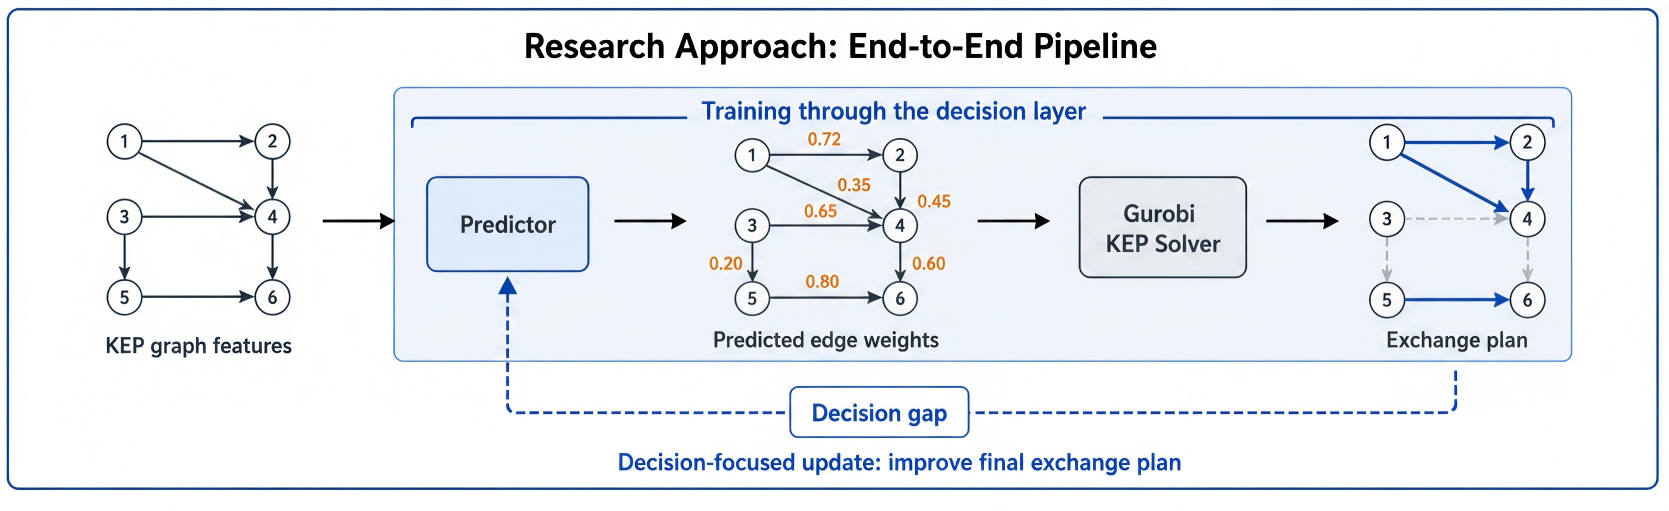
\includegraphics[width=0.98\textwidth]{figures/intern01/Research Approach.png}

  \vspace{-0.2em}
  \textbf{Solutions}

  \vspace{-0.2em}
  \begin{columns}[T,onlytextwidth]
    \begin{column}{0.48\textwidth}
      \textbf{\textcolor{kepred}{1. Surrogate gradients}}
      \begin{itemize}\setlength{\itemsep}{0em}
        \item Use a decision-focused surrogate loss.
        \item Convert discrete solver outputs into a usable training signal.
        \item FY perturbation is the main surrogate in this study.
      \end{itemize}
    \end{column}
    \begin{column}{0.48\textwidth}
      \textbf{\textcolor{keporange}{2. Gurobi model reuse}}
      \begin{itemize}\setlength{\itemsep}{0em}
        \item Reuse cycle/chain enumeration and model structure when possible.
        \item Update edge weights/objectives instead of rebuilding every solve.
        \item Reduce the cost of repeated solver-in-the-loop.
      \end{itemize}
    \end{column}
  \end{columns}

\end{frame}

\begin{frame}{Engineering Check: Solver Reuse Benchmark}
  \scriptsize
  \centering
  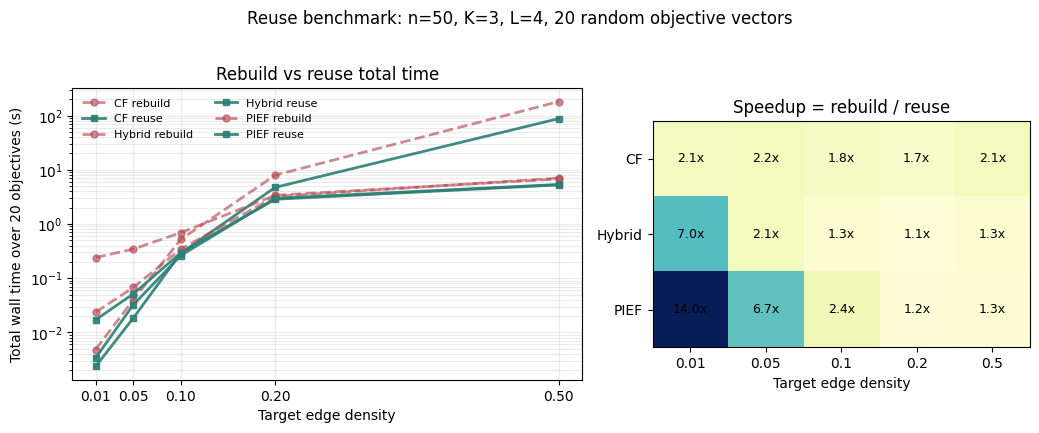
\includegraphics[width=0.86\textwidth]{figures/intern01/reuse_benchmark_speedup.png}

  \vspace{-0.25em}
  \begin{minipage}{0.92\textwidth}
    \textbf{Finding}
    \begin{itemize}\setlength{\itemsep}{0em}
      \item Reuse is faster in every formulation; gains are largest when model building dominates.
      \item Dense CF: \(181.2s \rightarrow 87.9s\); Hybrid/PIEF: about \(7s \rightarrow 5.3s\).
    \end{itemize}
  \end{minipage}
\end{frame}

\begin{frame}{Experiment Settings}
  \small
  \begin{block}{Purpose}
    Use a controlled two-dimensional setting to compare reward fitting with
    decision-focused surrogate training.
  \end{block}

  \vspace{0.45em}
  \begin{columns}[T,onlytextwidth]
    \begin{column}{0.47\textwidth}
      \textbf{Reward model}
      \[
        \hat w_e(\theta)=\theta_1 u_e+\theta_2 c_e
      \]
      \begin{itemize}\setlength{\itemsep}{0.45em}
        \item \(u_e\): edge utility feature.
        \item \(c_e\): recipient cPRA feature.
        \item \(\theta_1\): utility weight.
        \item \(\theta_2\): cPRA weight.
      \end{itemize}
    \end{column}
    \begin{column}{0.49\textwidth}
      \textbf{Synthetic label generation}
      \[
        w^{\mathrm{syn}}_e
        =
        \max\{0,\,(10u_e+5c_e)(1+\xi_e)\}
      \]
      \begin{itemize}\setlength{\itemsep}{0.45em}
        \item Noise-free coefficient: \([10,5]\).
        \item Multiplicative edge noise: \(\sigma=0.10\).
        \item Labels are synthetic edge benefits, not clinical outcomes.
      \end{itemize}
    \end{column}
  \end{columns}
\end{frame}

\begin{frame}{Experiment: Contour Landscapes}
  \scriptsize
  \begin{columns}[T,onlytextwidth]
    \begin{column}{0.62\textwidth}
      \centering
      {\tiny\textbf{\(\epsilon=0.2\)}}
      \vspace{-0.35em}
      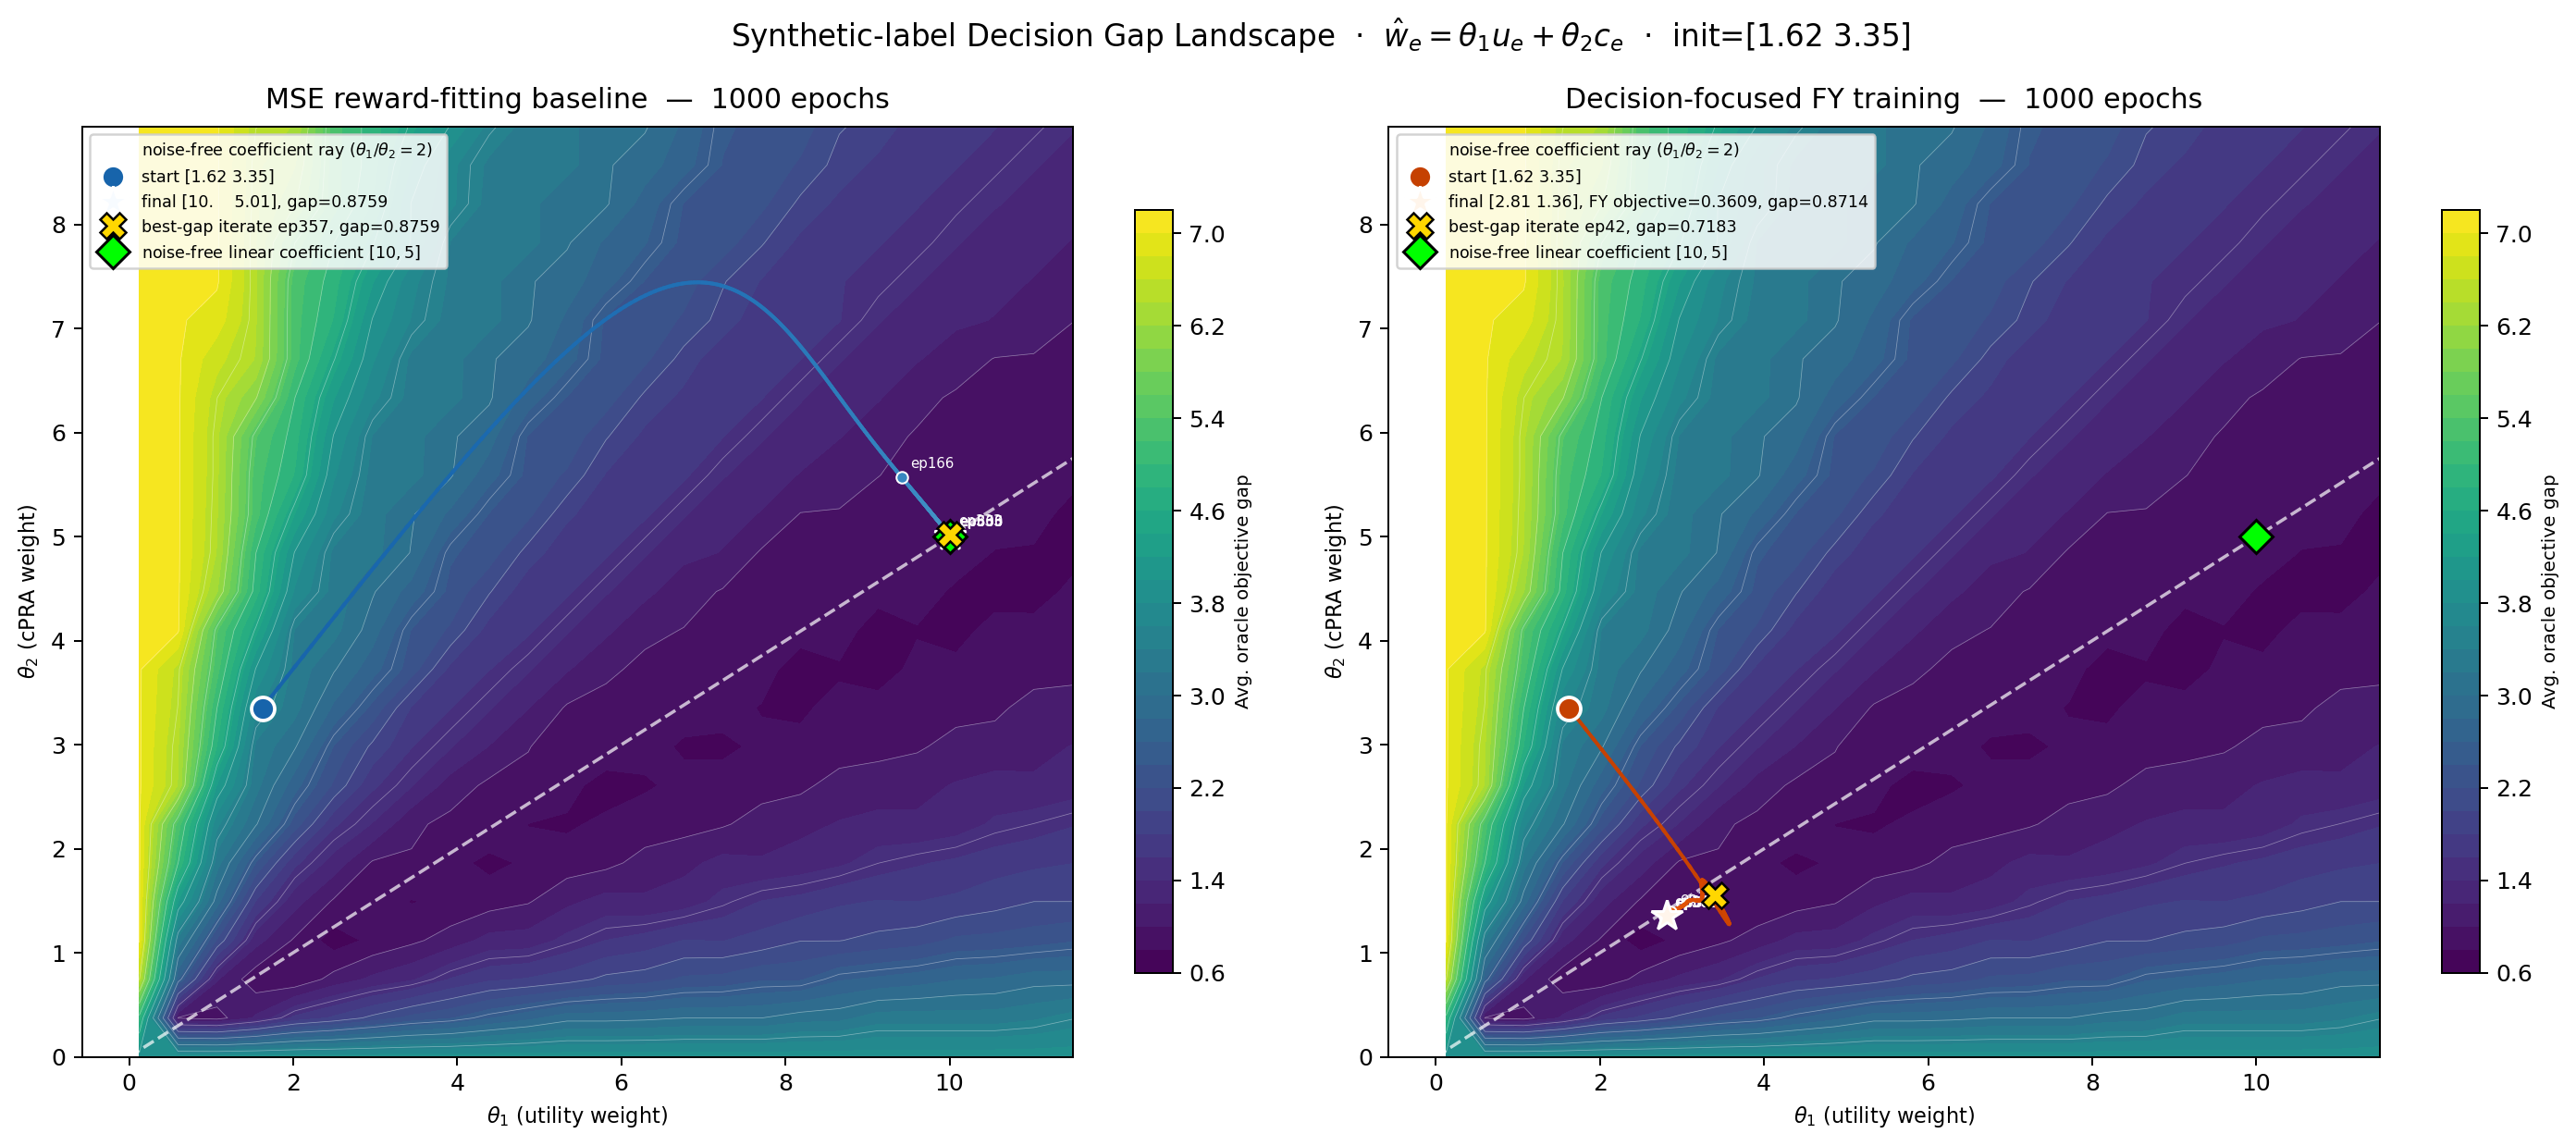
\includegraphics[height=0.36\textheight]{surrogate_experiment_results/Step1a/epsilon=0.2/trajectory_contour.png}

      \vspace{-0.35em}
      {\tiny\textbf{\(\epsilon=1.0\)}}
      \vspace{-0.35em}
      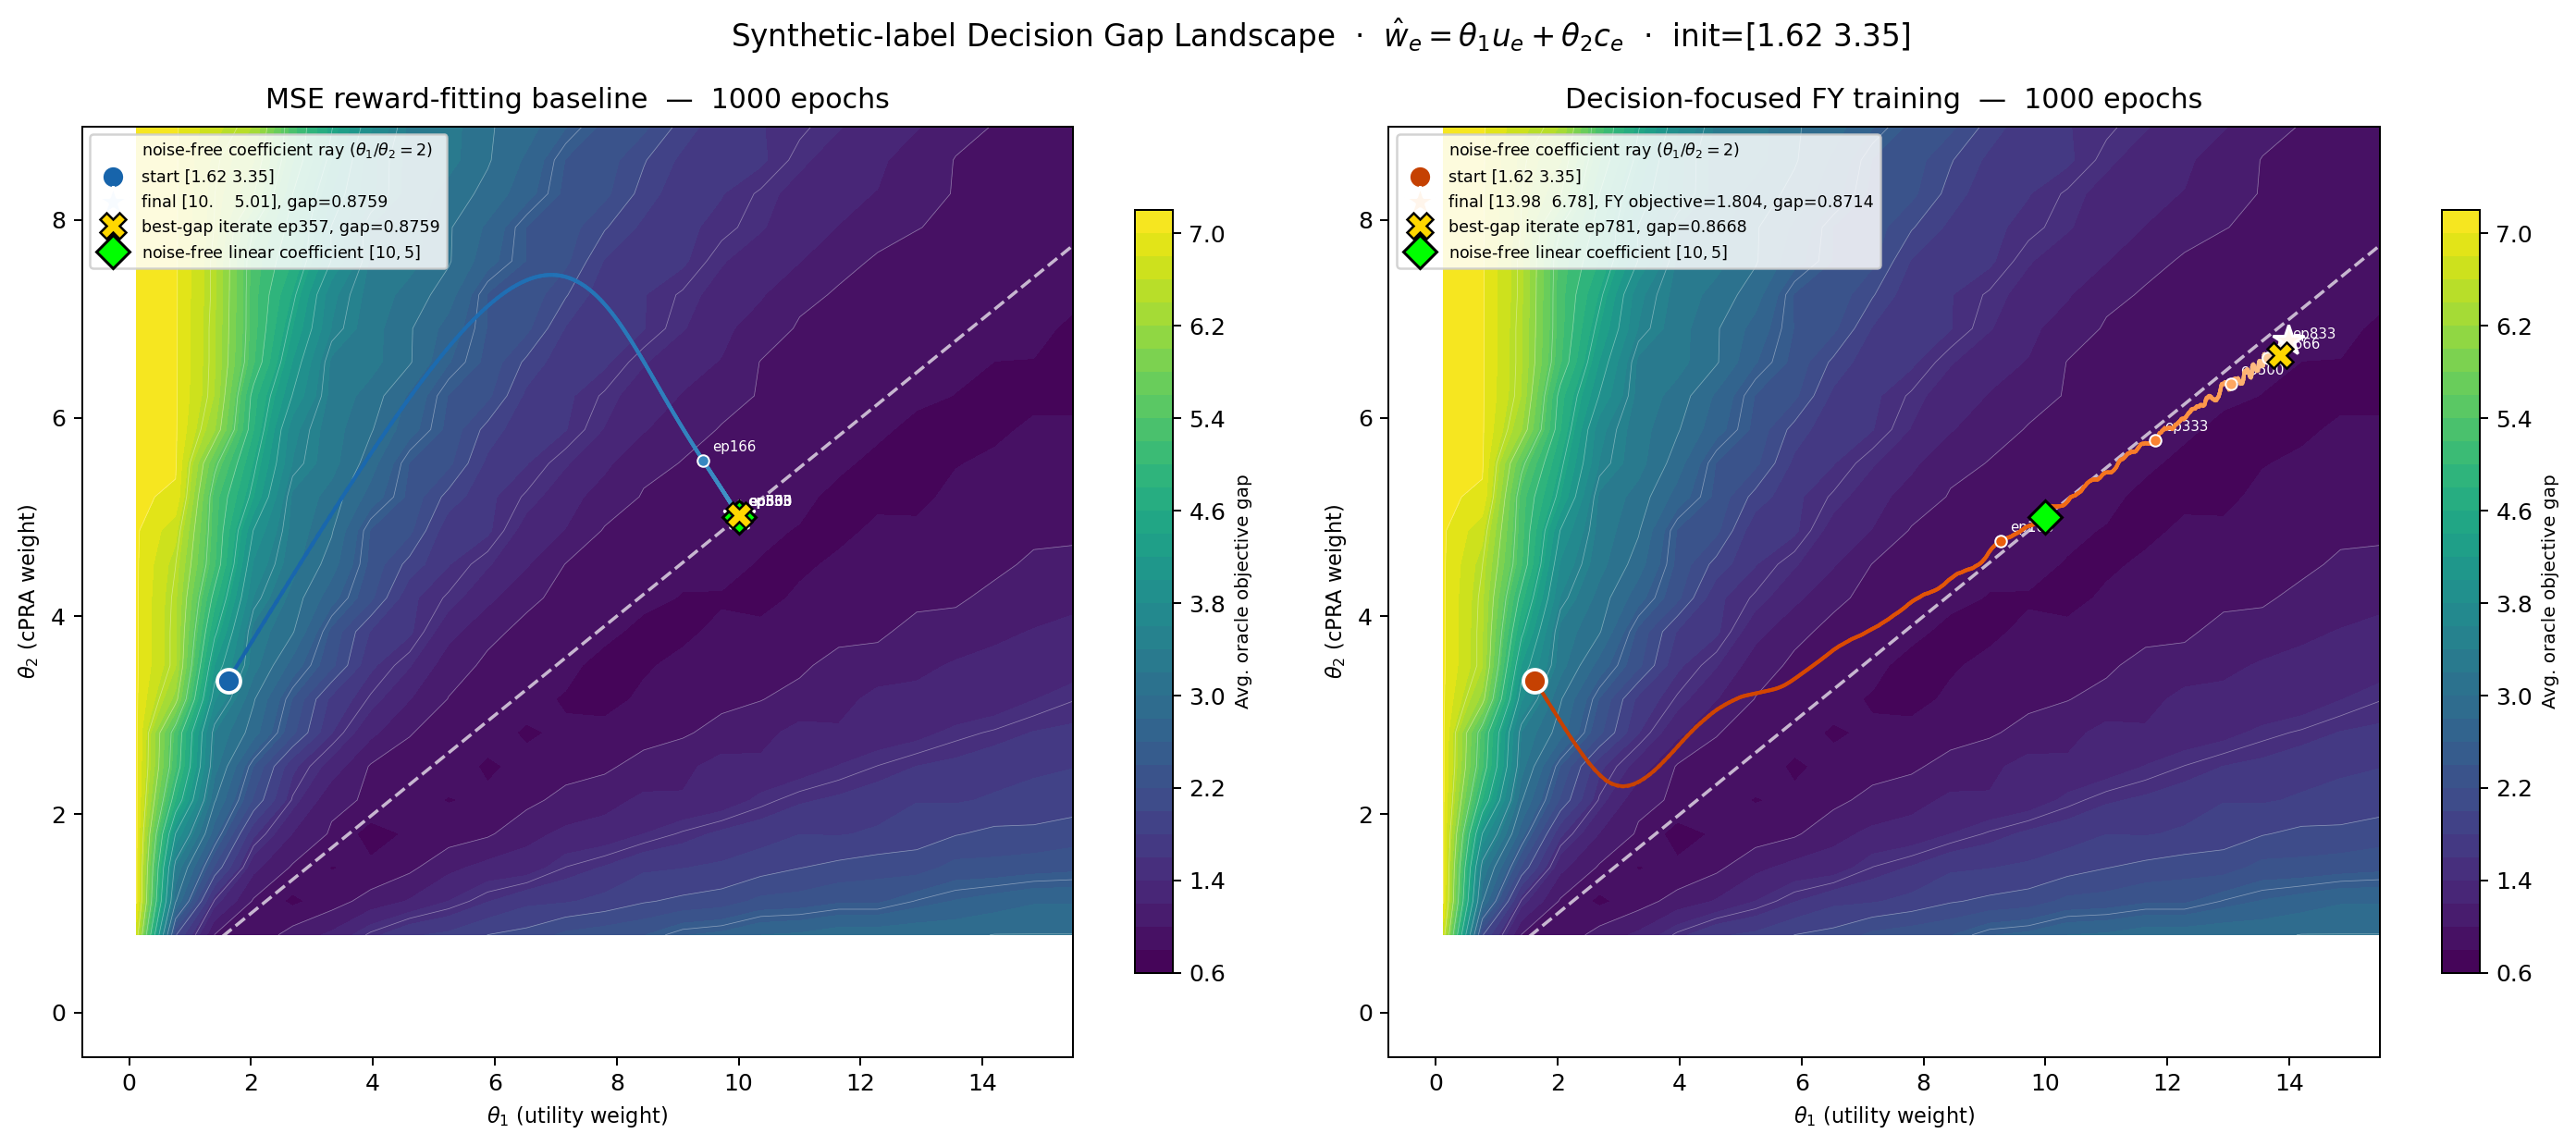
\includegraphics[height=0.36\textheight]{surrogate_experiment_results/Step1a/epsilon=1.0/trajectory_contour.png}
    \end{column}
    \begin{column}{0.36\textwidth}
      {\scriptsize\textbf{Observations}}
      {\small
      \begin{itemize}\setlength{\itemsep}{0.35em}
        \item MSE moves toward the clean-label direction \([10,5]\).
        \item FY follows a decision-induced path, not exact coefficient recovery.
        \item Smaller \(\epsilon\) gives a lower-scale FY endpoint.
        \item Both FY runs target decision quality rather than edge-level MSE fit.
      \end{itemize}
      }
    \end{column}
  \end{columns}
\end{frame}

\begin{frame}{Experiment: 3D Trajectories}
  \scriptsize
  \begin{columns}[T,onlytextwidth]
    \begin{column}{0.62\textwidth}
      \centering
      {\tiny\textbf{\(\epsilon=0.2\)}}
      \vspace{-0.35em}
      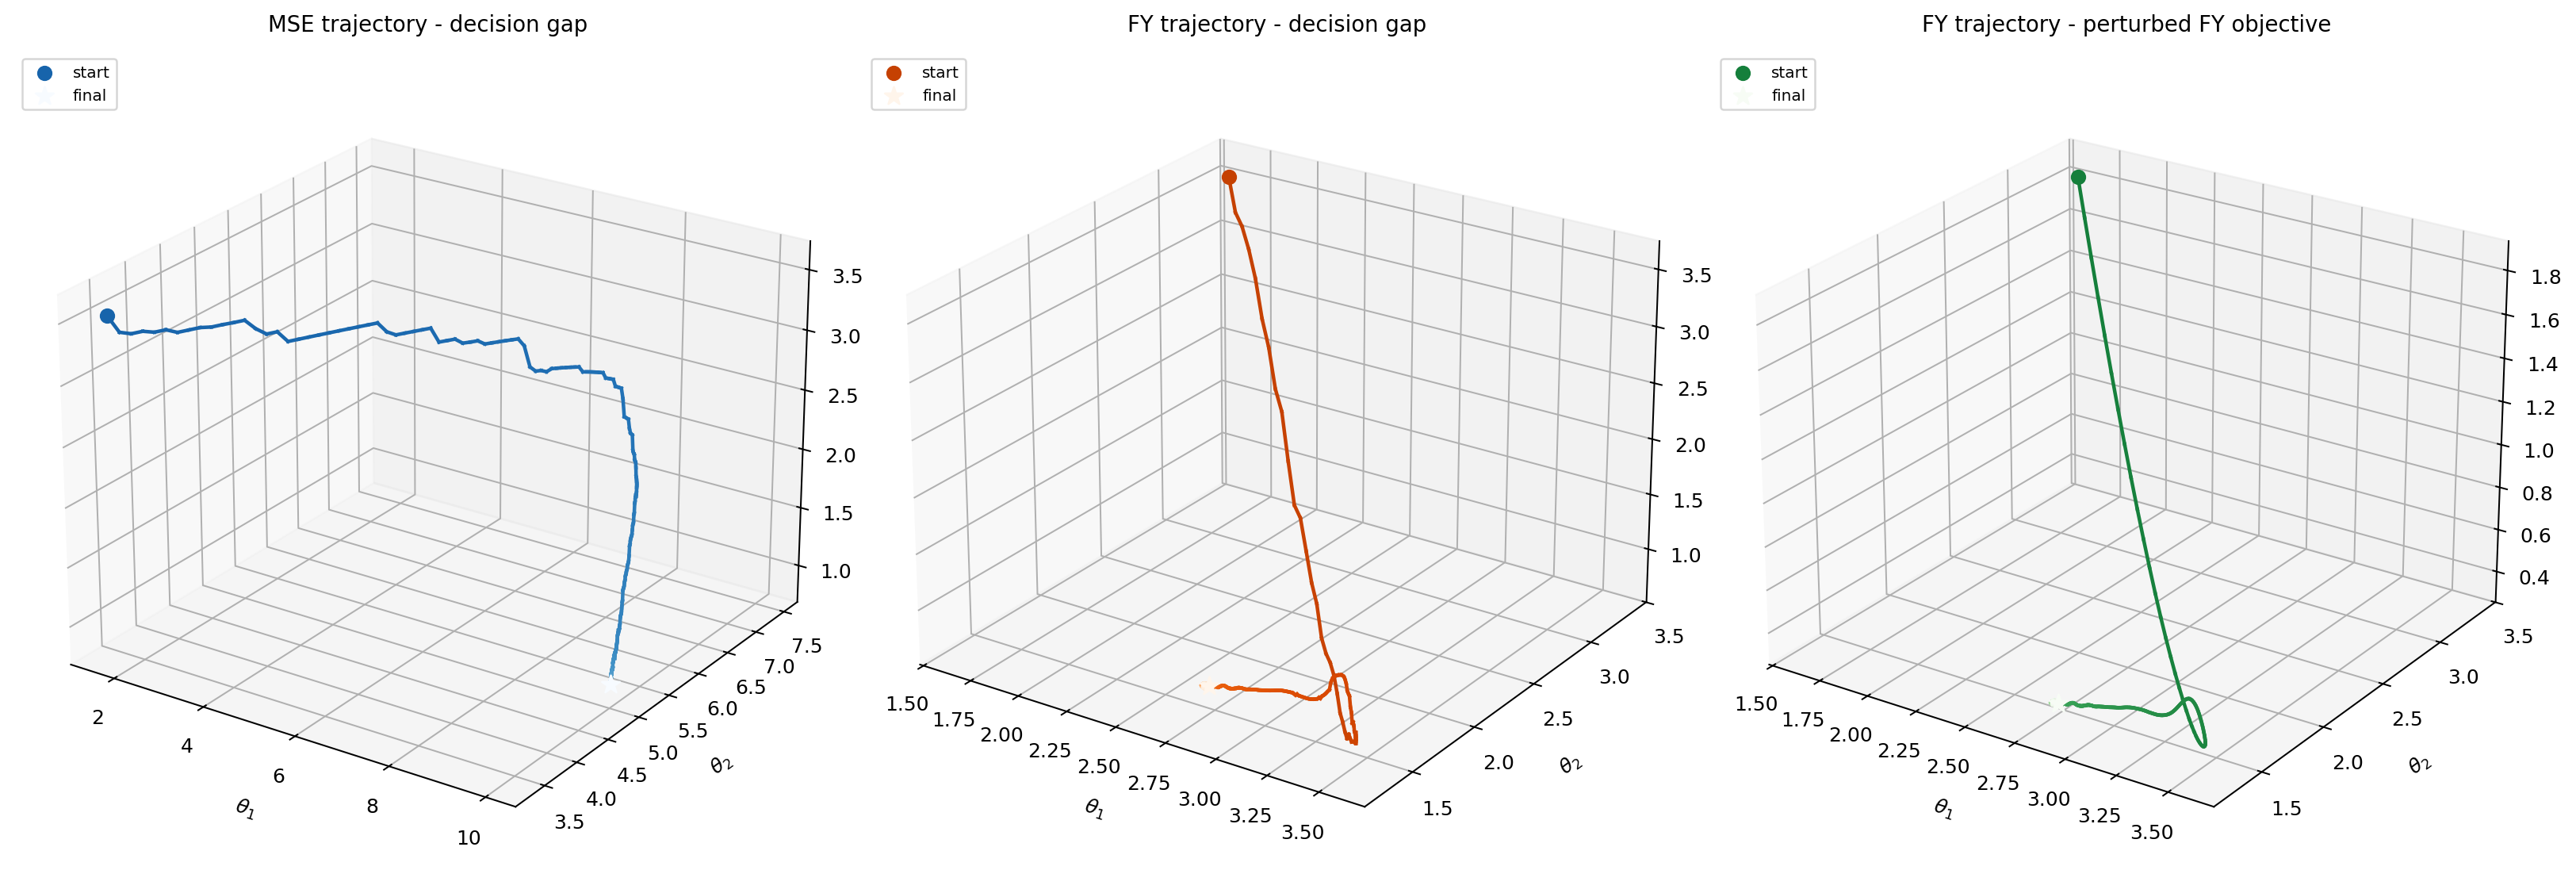
\includegraphics[height=0.36\textheight]{surrogate_experiment_results/Step1a/epsilon=0.2/trajectory_3d_metrics.png}

      \vspace{-0.35em}
      {\tiny\textbf{\(\epsilon=1.0\)}}
      \vspace{-0.35em}
      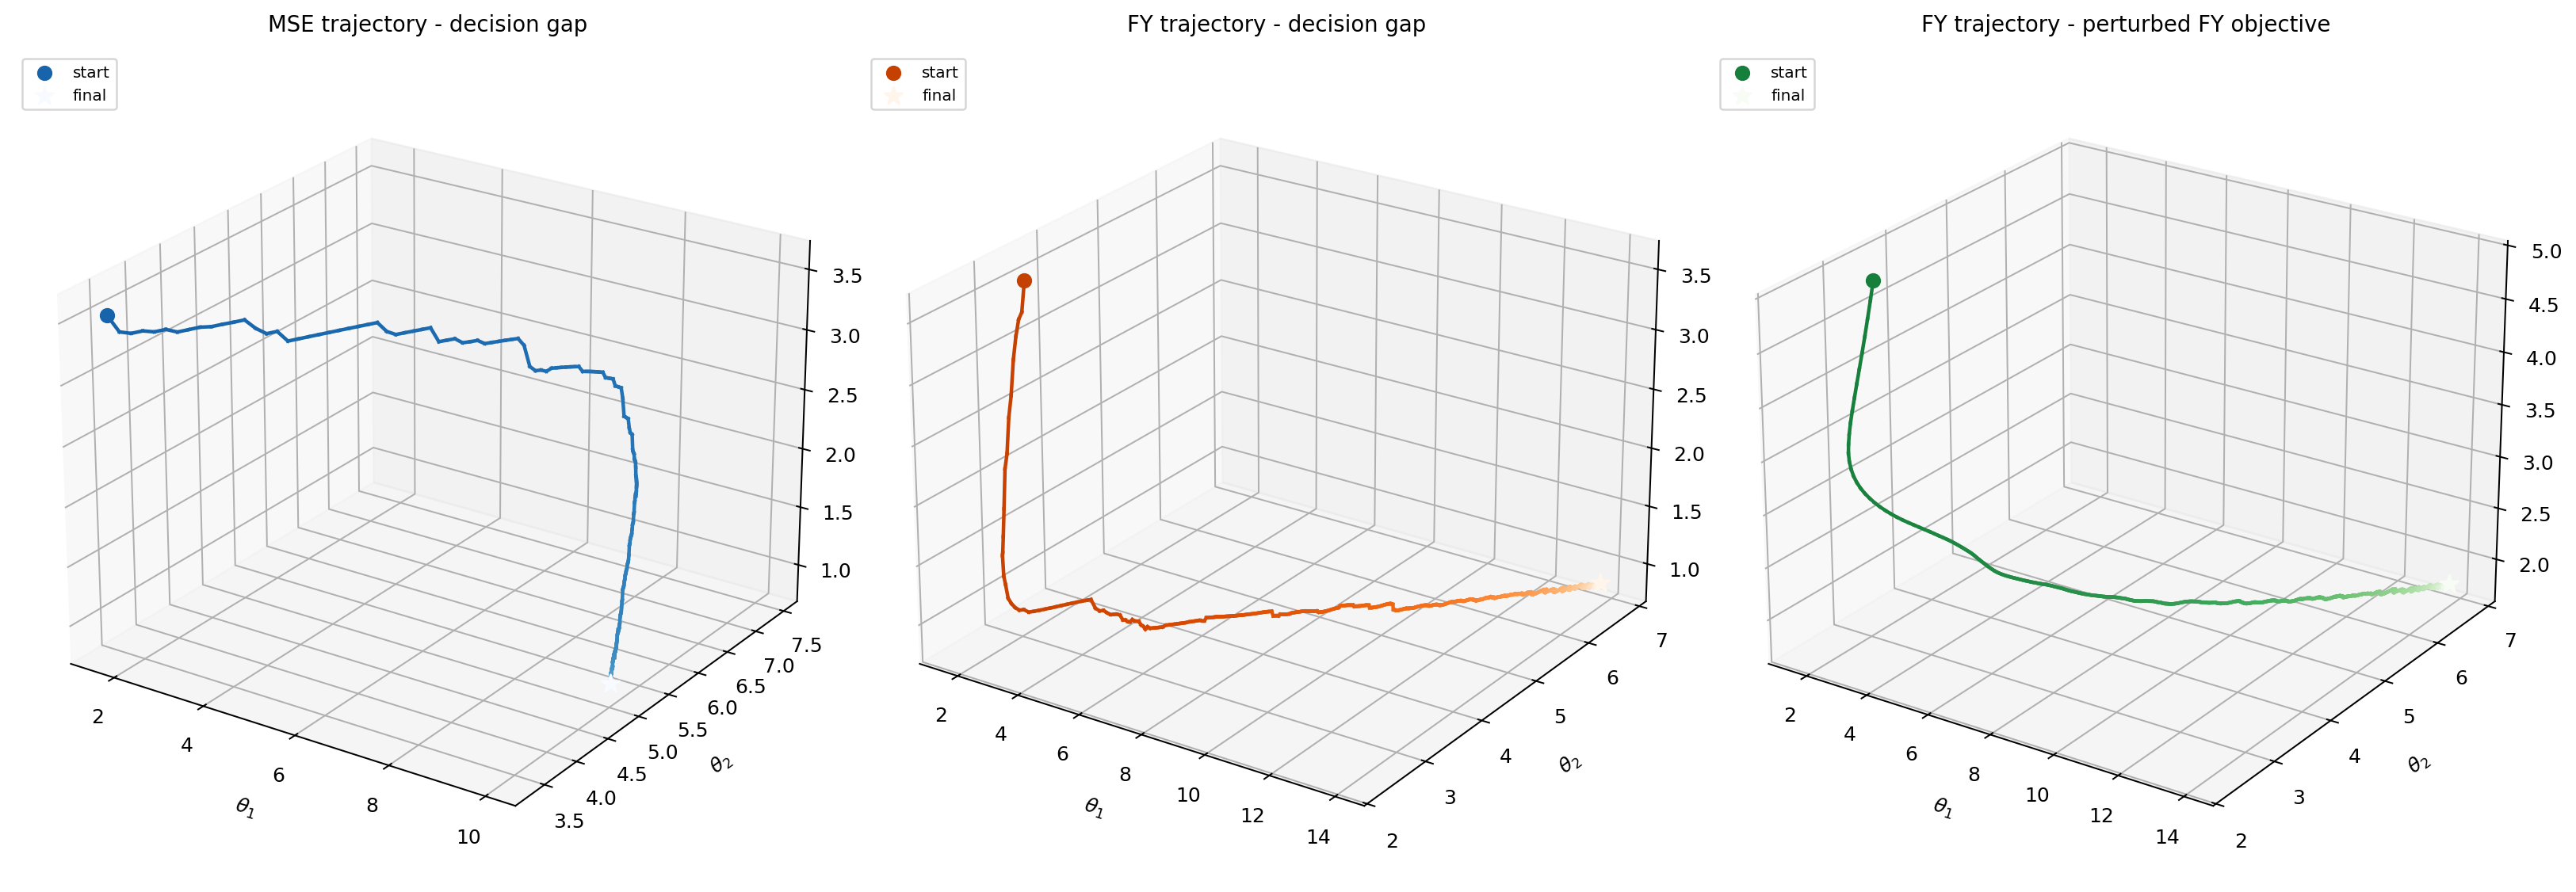
\includegraphics[height=0.36\textheight]{surrogate_experiment_results/Step1a/epsilon=1.0/trajectory_3d_metrics.png}
    \end{column}
    \begin{column}{0.36\textwidth}
      {\scriptsize\textbf{Observations}}
      {\small
      \begin{itemize}\setlength{\itemsep}{0.35em}
        \item 3D plots separate parameter motion from decision-gap and FY-objective changes.
        \item FY quickly moves toward a favorable region, then may plateau or oscillate.
        \item Decision gap and FY objective do not always improve monotonically together.
        \item The best decision-gap checkpoint can occur before the final epoch.
      \end{itemize}
      }
    \end{column}
  \end{columns}
\end{frame}

\begin{frame}{Experiment: Generalization Study}
  \begin{columns}[T,onlytextwidth]
    \begin{column}{0.34\textwidth}
      \scriptsize
      \textbf{Observations}
      \begin{itemize}\setlength{\itemsep}{0.35em}
        \item Metric: normalized decision gap; lower is better.
        \item FY-loss-selected E2E improves on the original held-out split.
        \item The advantage weakens on newly generated unseen graphs.
        \item Under realistic-synthetic label shift, two-stage is tied or better.
        \item The surrogate advantage depends on validation and distribution match.
      \end{itemize}
    \end{column}
    \begin{column}{0.64\textwidth}
      \centering
      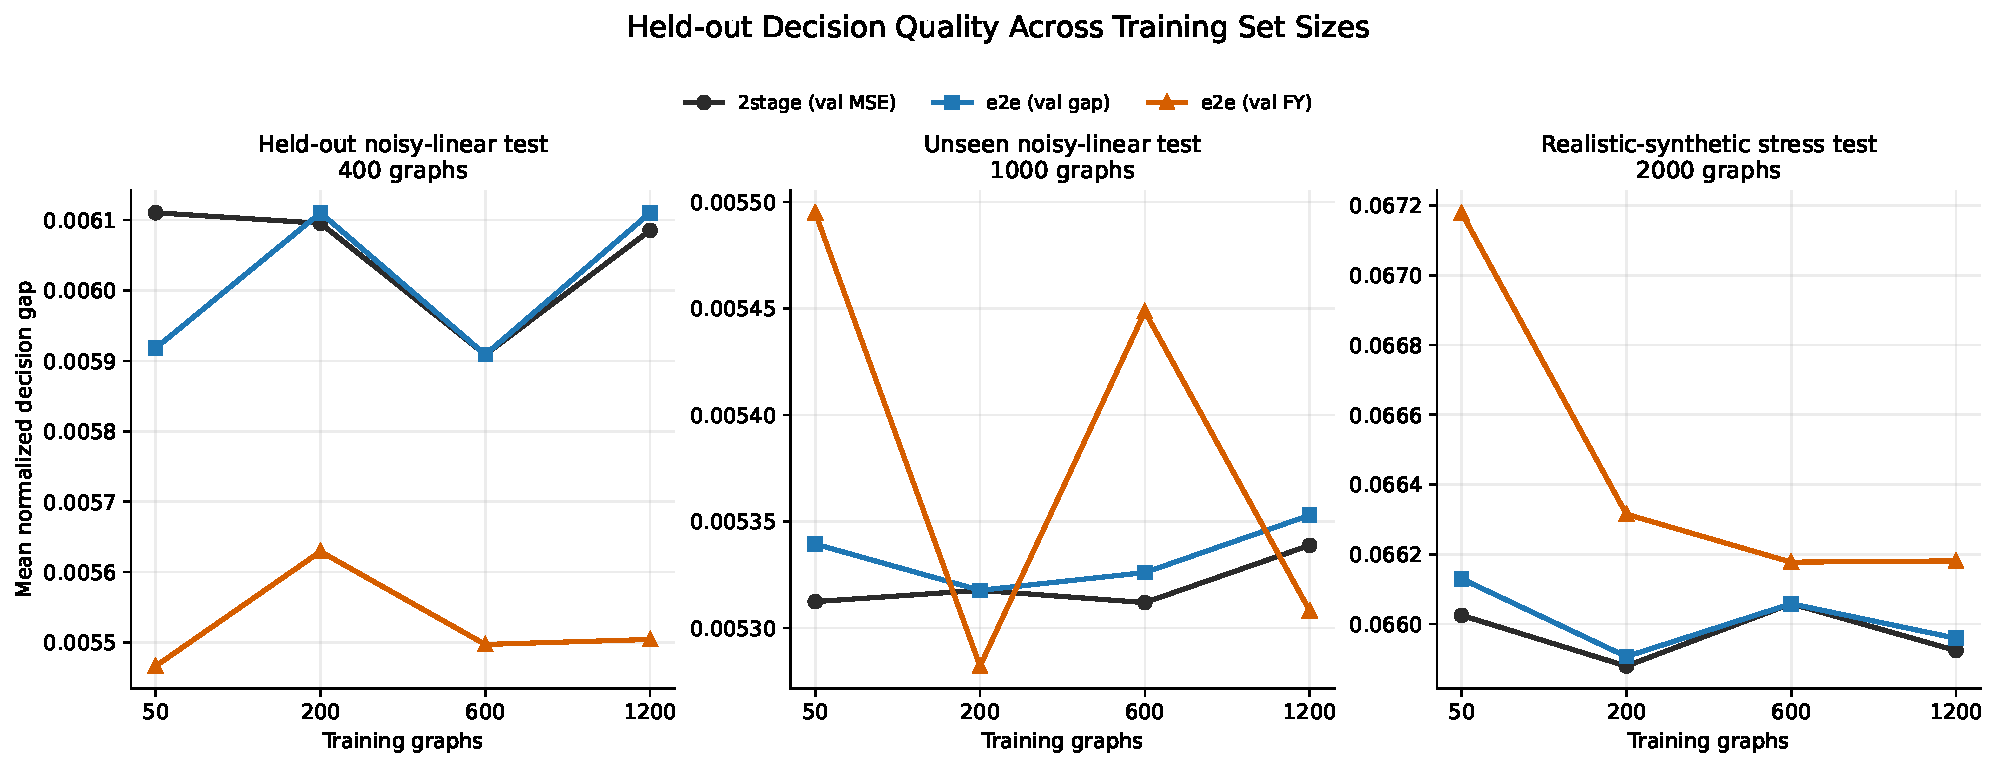
\includegraphics[width=\linewidth]{surrogate_experiment_results/Step1b/plot_results/01_normalized_decision_gap_by_dataset.pdf}
    \end{column}
  \end{columns}
\end{frame}

\begin{frame}{Additional Result: Full MLP/GNN KEP Pipeline}
  \scriptsize
  \centering
  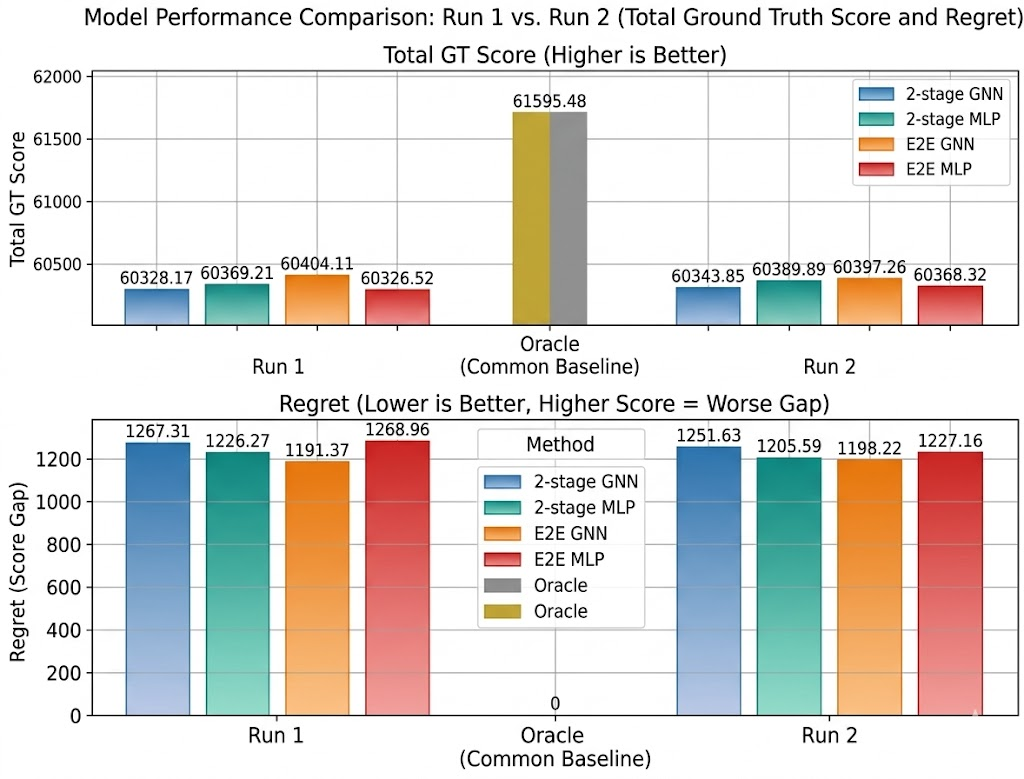
\includegraphics[width=0.86\textwidth,height=0.58\textheight,keepaspectratio]{Results.jpg}

  \vspace{-0.2em}
  \begin{minipage}{0.92\textwidth}
    \textbf{Observations}
    \begin{itemize}\setlength{\itemsep}{0em}
      \item Compared two-stage MLP/GNN, E2E MLP/GNN, and an oracle using ground-truth weights.
      \item E2E GNN gives modest repeatable gains over the two-stage GNN baseline.
      \item E2E MLP does not consistently improve over two-stage MLP; the oracle gap remains substantial.
    \end{itemize}
  \end{minipage}
\end{frame}

\section{Takeaways}

\begin{frame}{Takeaways: Promising, but Not Yet Robust}
  \centering
  \begin{minipage}{0.92\textwidth}
    \centering
    \large
    Decision-focused surrogate learning can improve controlled KEP decisions,\\
    but the gain is not automatic.
  \end{minipage}

  \vspace{1.0em}

  \scriptsize
  \begin{columns}[T,onlytextwidth]
    \begin{column}{0.29\textwidth}
      \begin{block}{What worked}
        \begin{itemize}\setlength{\itemsep}{0.35em}
          \item DFL changes the learned reward geometry.
          \item It can reduce downstream decision gap in controlled settings.
          \item It optimizes for final plans, not only edge prediction.
        \end{itemize}
      \end{block}
    \end{column}
    \begin{column}{0.29\textwidth}
      \begin{block}{Limitations}
        \begin{itemize}\setlength{\itemsep}{0.35em}
          \item Synthetic labels, not clinical outcomes.
          \item Simple two-feature Step1 probe.
          \item Limited seeds and distribution settings.
          \item Solver-in-the-loop training is expensive.
        \end{itemize}
      \end{block}
    \end{column}
    \begin{column}{0.29\textwidth}
      \begin{block}{Next steps}
        \begin{itemize}\setlength{\itemsep}{0.35em}
          \item Richer clinical edge-benefit models.
          \item Stronger GNN or structured predictors.
          \item Larger unseen tests and multiple seeds.
          \item Better surrogate validation strategy.
        \end{itemize}
      \end{block}
    \end{column}
  \end{columns}

  \vspace{0.8em}
  \colorbox{kepblue!8}{%
    \parbox{0.88\textwidth}{\centering\scriptsize
      \textbf{Conclusion:} useful signal in controlled benchmarks; robustness remains the key challenge.
    }%
  }
\end{frame}

\end{document}
